\documentclass{article}
\usepackage[margin=1in]{geometry}
\usepackage{amsmath,amsthm,amssymb}
\usepackage{bbm,enumerate,mathtools}
\usepackage{tikz,pgfplots}
\usepackage{chessboard}
\usepackage[hidelinks]{hyperref}
\usepackage{multicol} % Problem 35
\usepackage{xstring} % Difficulty command
\usetikzlibrary{shapes.geometric}

\newenvironment{question}{\begin{trivlist}\item[\textbf{Question.}]}{\end{trivlist}}
\newenvironment{note}{\begin{trivlist}\item[\textbf{Note.}]}{\end{trivlist}}
\newenvironment{references}{\begin{trivlist}\item[\textbf{References.}]}{\end{trivlist}}
\newenvironment{related}{\begin{trivlist}\item[\textbf{Related.}]\end{trivlist}\begin{enumerate}}{\end{enumerate}}

\newcommand\score[1]{
\pgfmathsetmacro\pgfxa{#1+1}
\tikzstyle{scorestars}=[
  star,
  star points=5,
  star point ratio=2.25,
  draw,
  inner sep=3pt,
  anchor=outer point 5
]
  \begin{tikzpicture}[baseline]
    \draw[opacity=0] (0,-0.5) rectangle (0,0.2); % Workaround for whitespace at the bottom.
    \foreach \i in {1,...,4} {
      \pgfmathparse{(\i<=#1?"yellow":"gray")}
      \edef\starcolor{\pgfmathresult}
      \draw (\i*4.5ex,0) node[name=star\i,scorestars,fill=\starcolor]  {};
    }
  \end{tikzpicture}
}

\newcommand{\difficulty}[1]{%
  \IfEqCase{#1}{%
      {1}{
        
\begin{tikzpicture}[scale=0.7, baseline=0.9mm]%
          \definecolor{slopegreen}{rgb}{0.0, 0.5, 0.0}%
          \fill[slopegreen] (0.5,0.5) circle (0.5);%
        \end{tikzpicture}%
      }%
      {2}{
        
\begin{tikzpicture}[scale=0.7, baseline=0.9mm]%
          \definecolor{slopeblue}{rgb}{0.0, 0.44, 1.00}
          \fill[slopeblue] (0,0) rectangle (1,1);%
        \end{tikzpicture}%
      }%
      {3}{
\begin{tikzpicture}[scale=0.7, baseline=0.9mm]\fill (0,0.5)--(0.5, 0)--(1,0.5)--(0.5,1)--cycle; \end{tikzpicture}}%
      {4}{
\begin{tikzpicture}[scale=0.7, baseline=0.9mm]\fill (0.25,0)--(0,0.5)--(0.25,1)--(0.5,0.5)--cycle; \fill (0.75,0)--(0.5,0.5)--(0.75,1)--(1,0.5)--cycle;\end{tikzpicture}}%
      % you can add more cases here as desired
  }[\PackageError{difficulty}{Undefined difficulty level: #1}{}]%
}%
\newcommand{\rating}[2]{\difficulty{#1}\\\score{#2}\\}


\begin{document}
  Consider ways to lay matchsticks (of unit length) on the $n \times m$ grid in
  such a way that no end is ``orphaned''.
  \begin{figure}[ht!]
    \centering
    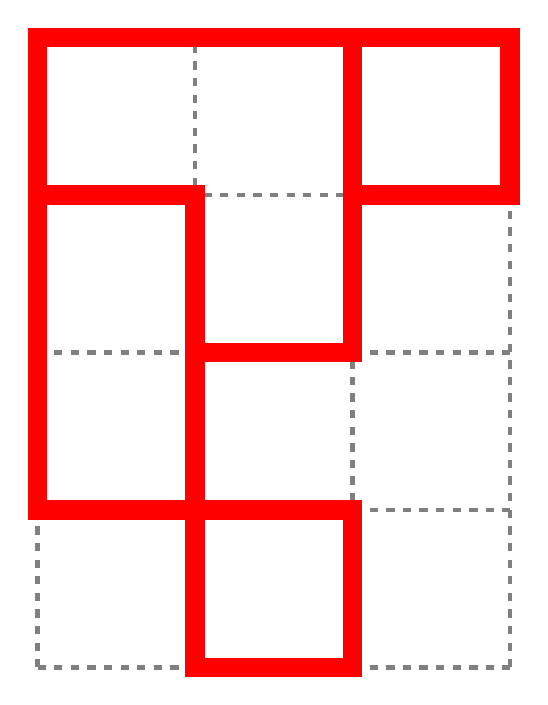
\begin{tikzpicture}[scale=2]
      \draw[ultra thick, gray, dashed] (0,0) grid (3,4);
      \draw[line width=0.25cm, red] (1,2)--(2,2)--(2,3);
      \draw[line width=0.25cm, red] (0,3)--(1,3)--(1,0)--(2,0)--(2,1)--(0,1)--(0,4)--(3,4)--(3,3)--(2,3)--(2,4);
    \end{tikzpicture}\hspace{1cm}
    \caption{
      An example of a valid configuration on a $3 \times 4$ grid.
    }
  \end{figure}
  \begin{figure}[ht!]
    \centering
    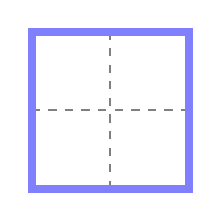
\begin{tikzpicture}
      \draw[thick, gray, dashed] (0,0) grid (2,2);
      \draw[line width=0.1cm, blue!50] (0,0) rectangle (2, 2);
    \end{tikzpicture}\hspace{0.5cm}
    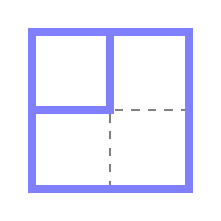
\begin{tikzpicture}
      \draw[thick, gray, dashed] (0,0) grid (2,2);
      \draw[line width=0.1cm, blue!50] (0,0) rectangle (2, 2);
      \draw[line width=0.1cm, blue!50] (0,1)--(1,1)--(1,2);
    \end{tikzpicture}\hspace{0.5cm}
    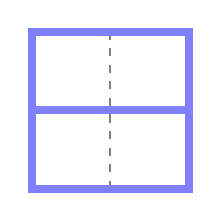
\begin{tikzpicture}
      \draw[thick, gray, dashed] (0,0) grid (2,2);
      \draw[line width=0.1cm, blue!50] (0,0) rectangle (2, 2);
      \draw[line width=0.1cm, blue!50] (0,1)--(2,1);
    \end{tikzpicture}\hspace{0.5cm}
    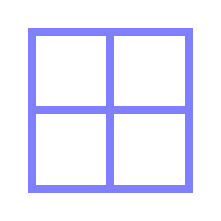
\begin{tikzpicture}
      \draw[thick, gray, dashed] (0,0) grid (2,2);
      \draw[line width=0.1cm, blue!50] (0,0) rectangle (2, 2);
      \draw[line width=0.1cm, blue!50] (0,1)--(2,1);
      \draw[line width=0.1cm, blue!50] (1,0)--(1,2);
    \end{tikzpicture}\hspace{0.5cm}
    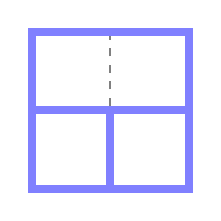
\begin{tikzpicture}
      \draw[thick, gray, dashed] (0,0) grid (2,2);
      \draw[line width=0.1cm, blue!50] (0,0) rectangle (2, 2);
      \draw[line width=0.1cm, blue!50] (0,1)--(2,1);
      \draw[line width=0.1cm, blue!50] (1,0)--(1,1);
    \end{tikzpicture}
    \caption{
      All(?) examples of valid configurations of $2 \times 2$ grids with
      border, up to dihedral action.
    }
  \end{figure}
  \begin{question}
    Let $a_\ell(n)$ be the number of configurations on the $\ell \times n$ grid.
    What is a general formula for $a_\ell(n)$?
  \end{question}

  \begin{related}
    \item What if the matchsticks are of length $k$?
    \item How does this generalize to a triangular/hexagonal lattice or to
      multiple dimensions?
    \item What is the number of these configurations with rotational symmetry?
      Horizontal/vertical symmetry?
    \item If such a configuration is chosen uniformly at random, what is the
      number of expected regions? (e.g. the first example has 4 interior
      regions.)
  \end{related}
\end{document}
